% プロジェクト学習中間報告書書式テンプレート ver.1.0 (utf8)

% 両面印刷する場合は `openany' を削除する
\documentclass[11pt,papersize]{jsbook}

% 報告書提出用スタイルファイル
%\usepackage[final]{funpro}%最終報告書
\usepackage[middle]{funpro}%中間報告書

% 画像ファイル (EPS, EPDF, PNG) を読み込むために
\usepackage[dvipdfmx]{graphicx,color}

% ファイル分割のためのパッケージ
\usepackage{subfiles}

% ここから -->
\usepackage{calc,ifthen}
\newcounter{hoge}
\newcommand{\fake}[1]{\whiledo{\thehoge<70}{#1\stepcounter{hoge}}%
  \setcounter{hoge}{0}}
% <-- ここまで 削除してもよい

% 年度の指定
\thisYear{2017}

% プロジェクト名
\jProjectName{ビーコンIoTで函館のまちをハックする}

% [簡易版のプロジェクト名]{正式なプロジェクト名}
% 欧文のプロジェクト名が極端に長い(2行を超える)場合は、短い記述を
% 任意引数として渡す。
%\eProjectName[Making Delicious curry]{How to make delicious curry of Hakodate}
\eProjectName{Leverage the Beacon IoT in Hakodate Real Downtown for Our Smarter Life}


% <プロジェクト番号>-<グループ名>
\ProjectNumber{8-B}

% グループ名
\jGroupName{Youbeacomm}
\eGroupName{Youbeacomm}

% プロジェクトリーダ
\ProjectLeader{1015253}{橋場保鷹}{Hodaka~Hashiba}

% グループリーダ
\GroupLeader  {1015215}{藤原祐汰}{Yuta~Fujiwara}

% メンバー数
\SumOfMembers{5}
% グループメンバ
\GroupMember  {1}{1015074}{河田歩美}{Ayumi~Kawada}
\GroupMember  {2}{1015215}{藤原祐汰}{Yuta~Fujiwara}
\GroupMember  {3}{1015240}{荒田啓太郎}{Keitaro~Arata}
\GroupMember  {4}{1015250}{高橋大輔}{Daisuke~Takahashi}
\GroupMember  {5}{1015253}{橋場保鷹}{Hodaka~Hashiba}


% 指導教員
\jadvisor{松原克弥,藤野雄一,鈴木恵二,奥野拓}
% 複数人数いる場合はカンマ(,)で区切る。カンマの前後に空白は入れない。
\eadvisor{Katsuya~Matsubara,Yuichi~Fujino,Keiji~Suzuki,Taku~Okuno}

% 論文提出日
\jdate{2017年7月21日}
\edate{July~21, 2017}

\begin{document}
%
% 表紙
\maketitle

%前付け
\frontmatter

% 和文概要
\begin{jabstract}

% プロジェクト全体の日本語概要
\subfile{mid-report-common/common-jabstract}

グループBは、フィールドワークから外国人観光客への言語の対応が必要と考え、外国人観光客が日本人とスムーズに会話できるように手助けをするためのスマートフォン向けのアプリケーションを作成することを目的とした。この問題を解決するために指さし会話帳というものがある。しかし既存の指さし会話帳では、自分が欲しいフレーズをすぐ見つけられない、欲しいフレーズが掲載されていないなどの課題がある。ここから、ビーコンで利用者のコンテキストを読み取り、そこから欲しい情報をしスマートフォンにアプリケーションから送信するというサービスを提案した。
しかしこの提案を7月14 日に行われた中間報告会で発表したところ、たくさんの課題が見つかった。後期では課題をもとにグループで提案を改善しアプリケーションを作成をする。そのアプリケーションを実際に外国人観光客に使用してもらい、レビューをいただく予定である。そしてこれを繰り返すことで外国人観光客のコミュニケーションを支援する。

% 和文キーワード
\begin{jkeyword}
  ビーコン, 函館, 外国人観光客, 指さし会話帳, コンテキスト
\end{jkeyword}
\bunseki{藤原祐汰}

\end{jabstract}

%英語の概要
\begin{eabstract}

% プロジェクト全体の英語概要
\subfile{mid-report-common/common-eabstract}

 Group B considers that language response from fieldwork to foreign tourists is necessary and aims to help foreign tourists to talk with Japanese smoothly. I thought that this problem would be solved by dissemination of existing pointing speech book. However, in the existing pointing conversation book, there is a problem that you can not find the phrase you want immediately, and the phrase you want is not posted. From here, in group B, we propose a service that makes existing pointing conversation book a smartphone application, reads the situation of the user with beacon, senses the information desired from it, and sends it from the application to the smartphone. However, when this proposal was announced at the interim report meeting held on July 14, a lot of subjects were found. In the latter term, we will improve the proposal by the group based on the task and create a prototype. I will have the prototype actually used by foreign tourists and will be reviewed. And by repeating this we support communication of foreign tourists.

% 英文キーワード
\begin{ekeyword}
  Beacon, Hakodate, Foreign Tourists, Pointing Conversation Book, Context
\end{ekeyword}
\bunseki{藤原祐汰}

\end{eabstract}

\tableofcontents% 目次


\mainmatter% 本文のはじまり

% プロジェクト共通の項目
\subfile{mid-report-common/common-chapters}


% グループごとの項目
\chapter{サービスの提案にあたって}

\section{背景}

\subsection{函館に訪れる外国人観光客}
 函館市は、北海道の中にある市の一つで人口はおよそ26万人の都市である。函館市は夜景や歴
史的建造物、温泉といった多くの観光地を持っているため、日本人だけではなく多くの外国人観光
客が訪れる。平成28年度における観光入込客数は、上期(4月9月)は約366万5千人
(前年同期に比べ約45万4千人増の114.1%)、下期(10月3月)は約194万2千人(約20万6千人増の111.9%)、合計約560万7千人(約66万人増の113.3%)となった。さらに
外国人宿泊客数については、台湾や中国だけでなく、近年はタイ、マレーシアなどの東南アジアか
らの宿泊客が増加し、全体でも約40万5千人(約7千人増、前年比101.9%) と過去最高を
更新した\cite{b}。
以上のことから、現在函館には多くの外国人観光客が訪れていることがわかる。しかし、外国人が函館を観光する上でさまざまな問題を抱えている。
\bunseki{藤原祐汰}

\subsection{函館の地元民と外国人観光客の意思疎通の問題}\label{sec:mokuteki}
 毎年多くの外国人観光客が訪れる中での問題点は、地元民がどう他言語に対応するかという問題である。母国語で話をしてくる外国人観光客が、何を伝えたいのか理解するのが難しく、同じ言語で会話するレベルでの意思疎通を図ることは非常に困難である。ここで情報センター出版局で出版されている「旅の指さし会話帳」(以下、指さし会話帳)というものがある。指差し会話帳とは、旅行中で頻繁に使われるフレーズが、日本語と外国語に訳されており、指をさすだけでコミュニケーションがとれるという会話集のことである。
この本は現在70以上の言語に対応できるようにシリーズ化されている。しかし既存の「指さし会話帳」には扱いにくい点が2 つある。
1 つ目は、掲載されているフレーズ多いということである。そのために、自分の伝えたいフレーズがどこに掲載されているのかわからず、本の扱いに慣れるまでは見つけにくいという点である。
2 つ目は、掲載されているフレーズしか使えない点である。つまり本のなかに利用者のほしいフレーズがない場合、的確なコミュニケーションをとることができなのである。
\bunseki{藤原祐汰}

\section{目的}
 本グループは~\ref{sec:mokuteki}~で取り上げた既存の「指さし会話帳」の課題をビーコンIoTで改善しスマートフォン向けのアプリ「Youbeacomm」指さし会話帳を改良・発展させたものを作成する。このアプリを外国人観光客が利用することで、函館に訪れる外国人観光客と函館民のコミュニケーションの手助けをすることを目的とする。
\bunseki{藤原祐汰}


\chapter{Youbeacommについて}

\section{Youbeacommの概要}
 Youbeacommは外国人旅行者と日本人をつなぐコミュニケーション促進サービスとして、お互いに共通の言語がない人々に対し、そのコミュニケーションをソフトウェアによって支援する。
同様の課題への解決策として、「旅の指さし会話帳」という、様々なフレーズや単語が2言語で併記されている書籍が市販されている。
外国人旅行者はこの書籍に印刷されたフレーズや単語を指さすだけで、気軽に現地の人とコミュニケーションを行うことができる。
旅行中の様々な場面で使われていることを想定しているため、コンテンツは非常に充実しており、日常で発生するであろう大半のケースに対応している。
しかしながら、掲載されている情報量が多いことのデメリットとして、旅行先での各場面ごとに適切な情報を絞り込むことが困難であることがあげられる。
また、紙媒体である以上、同一のコンテンツを重複して掲載することは難しく、利用者の想像と全く異なるジャンルのページに掲載されていることもある。
例として、写真を撮ってもらいたい場合に使うフレーズが観光に関連するすべてのページ掲載されていれば、ページめくりは発生しないが、
実際には持ち運びやすい判型にするという紙面の都合上、「あいさつ」というジャンルに分類されている。

本提案手法では利用者の現在地や移動経路、時間帯、天候など、コミュニケーションで支援が必要となる状況に至った要素と、
あらかじめ収集した場所の属性(商業施設、駅、市役所など)やその周辺の状況などを総合して、「コンテキスト」と呼び、それらの情報を数値化する。
それらを基に利用者の置かれている環境を把握し、フレーズや単語の絞り込みや優先度付けを行うことで、利用者がその時点で正に求めている候補を提案することを目指す。
例として、利用者が空港の搭乗口と到着ロビーへ順に接近 (設置したビーコンを検知) したとする。
その場合、「空港に到着した後、ターミナル外に移動しようとしている」ものとして、路線バスやタクシーなどの移動手段についてのフレーズが求められるであろうと推定できるため、
交通に関係するフレーズを絞り込み、空港からの移動手段を優先的に表示することなどが考えられる。
\begin{center}
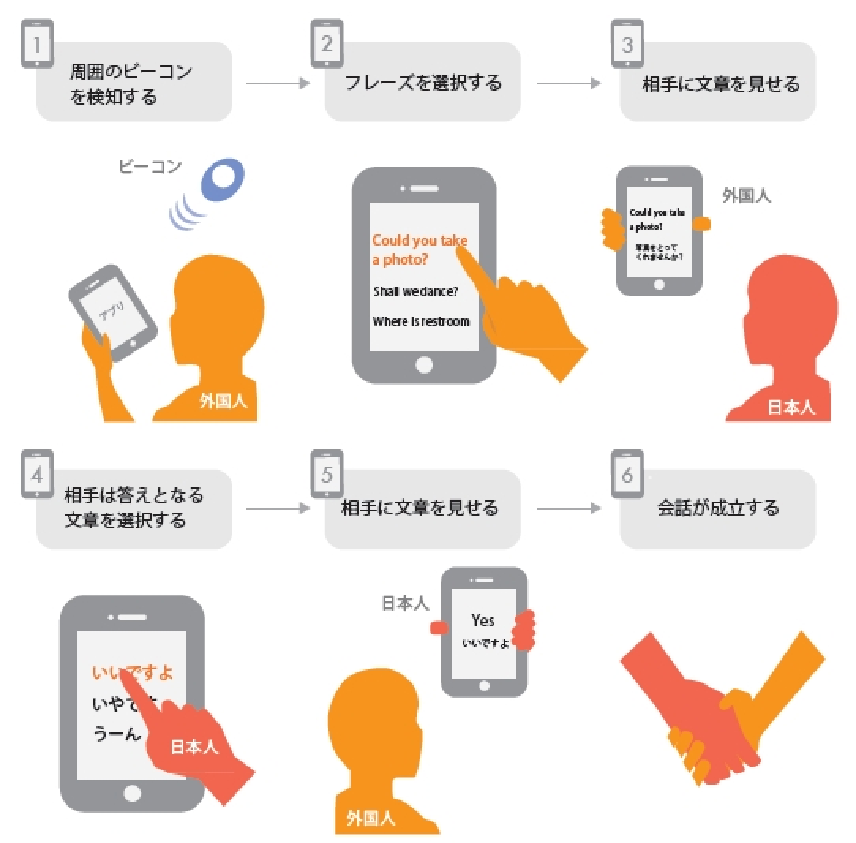
\includegraphics[width=10cm]{abc.pdf}\\
提案するサービス
\end{center}
\bunseki{高橋大輔}

\section{Youbeacommの具体的なシステムの説明}
 本システムへのアクセスは外国人旅行者向けのスマートフォンのアプリとして提供する。米Net Applications社のマーケットシェア調査\cite{b}によると、
世界の携帯端末の97.12%以上はAndroid (64.20%) かiOS (32.92%) を実行していることから、これら2つのOSを開発ターゲットとする。
アプリはGPS、(設置するビーコンを含む) Bluetooth Low Energy、Wi-Fiなどの情報をバックグラウンドで定期的に取得し、
利用者の起動操作によって、フォアグラウンドとなった時点で、それらの情報をサーバに送信する。
サーバはそれらを基に位置情報や利用者周辺の環境を推定し、コンテキストを認識する。データベースに登録されているフレーズのうち、そのコンテキストにマッチするものを抜き出し、
コンテキストとフレーズの関係から優先度を計算して並び替えたリストを、アプリに対して応答することで、利用者に対してフレーズの提案が行われる。
利用者が提案されたフレーズから適切なものを選択すると、そのフレーズが2か国語で表示され、コミュニケーションの相手 (日本語話者を想定) に提示したのち、スマートフォンを相手に渡す。
サーバは選択された発話フレーズをコンテキストの1つとして考慮した上で、同様にデータベースからフレーズを提案し、その中から適切な回答を選択してもらう。
提案の中に適切なフレーズがない場合には、機械翻訳や観光案内所、電話による通訳サービスなどの案内を行うようにすることで、
利用者に対して常に複数の選択肢を提供しつつ、データの充実を主な目的として、これらのサービスとの様々な連携も行う。
また、適切なフレーズの提案がなかったこと自体については、提案されたフレーズに対して、利用者がフィードバックや追加の提案を行えるようにすることで、
フレーズの充実、並びに提案精度の向上を図る。
ビーコンなどの情報から位置情報等を推定するシステムには、簡易的なビーコンの遠隔監視の役割を持たせる。
ビーコンが各利用者のスマートフォンに検知された事実や、ビーコンから一定の割合で通知される電池残量などの情報を、アプリを介して収集し、
検知された頻度や電池残量の推移などの得られた情報を用いて、状態異常などを早期に把握し、効率的なメンテナンスの計画を立案するための情報源とする。
\begin{figure}[htbp]
 \begin{center}
  \makebox[\textwidth]{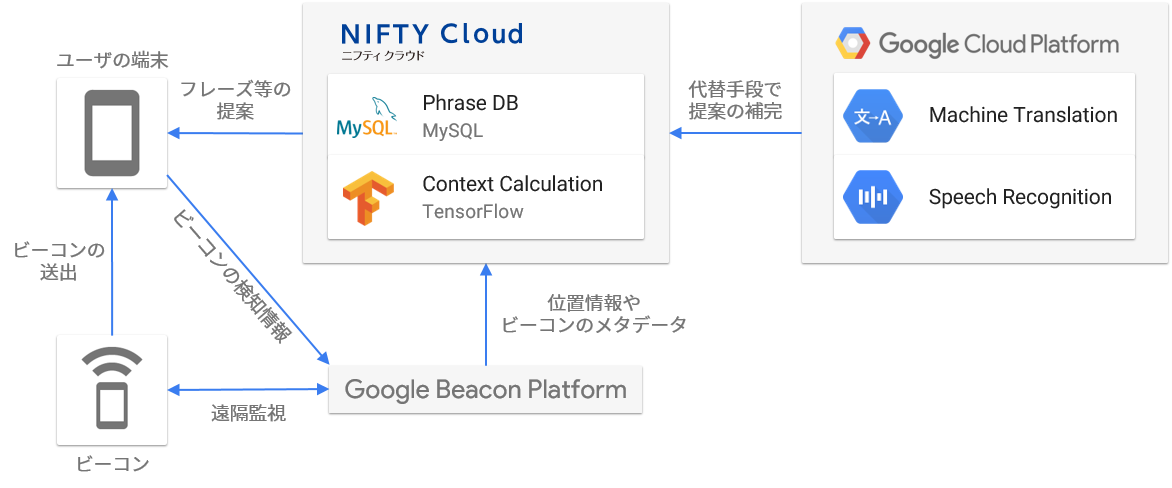
\includegraphics[width=0.75\paperwidth]{system_structure.png}}
 \end{center}
 \caption{システム構成図}
 \label{fig:one}
\end{figure}
\bunseki{高橋大輔}

\section{現時点でのプロトタイプ}\label{sec:sannosan}
 中間報告会での説明のツールを兼ね、主要な機能の画面遷移を再現した14画面で構成される静的なプロトタイプの制作を行った。
このプロトタイプでは、アプリのインストールに誘導するプロモーションや実際のインストールなど、アプリの起動に至るまでのプロセスや、観光案内所などへの誘導のプロセスなどが
未再現ではあるものの、プロトタイピングツールを用いて制作する過程で、メンバー間でのアプリの機能に対する細部の認識を共有することができた。
今後、このプロトタイプをベースとして、動的にフレーズを提案する機能などを盛り込んだプロトタイプを制作したのち、その他の機能を順次実装していく。
その過程で、実際の外国人旅行者に使用・評価してもらい、利用者への理解を深め、プロトタイプを制作するというプロセスを繰り返すことで、
利用者にとって最適なUXを提供できるシステムに近づけていく。
\begin{center}
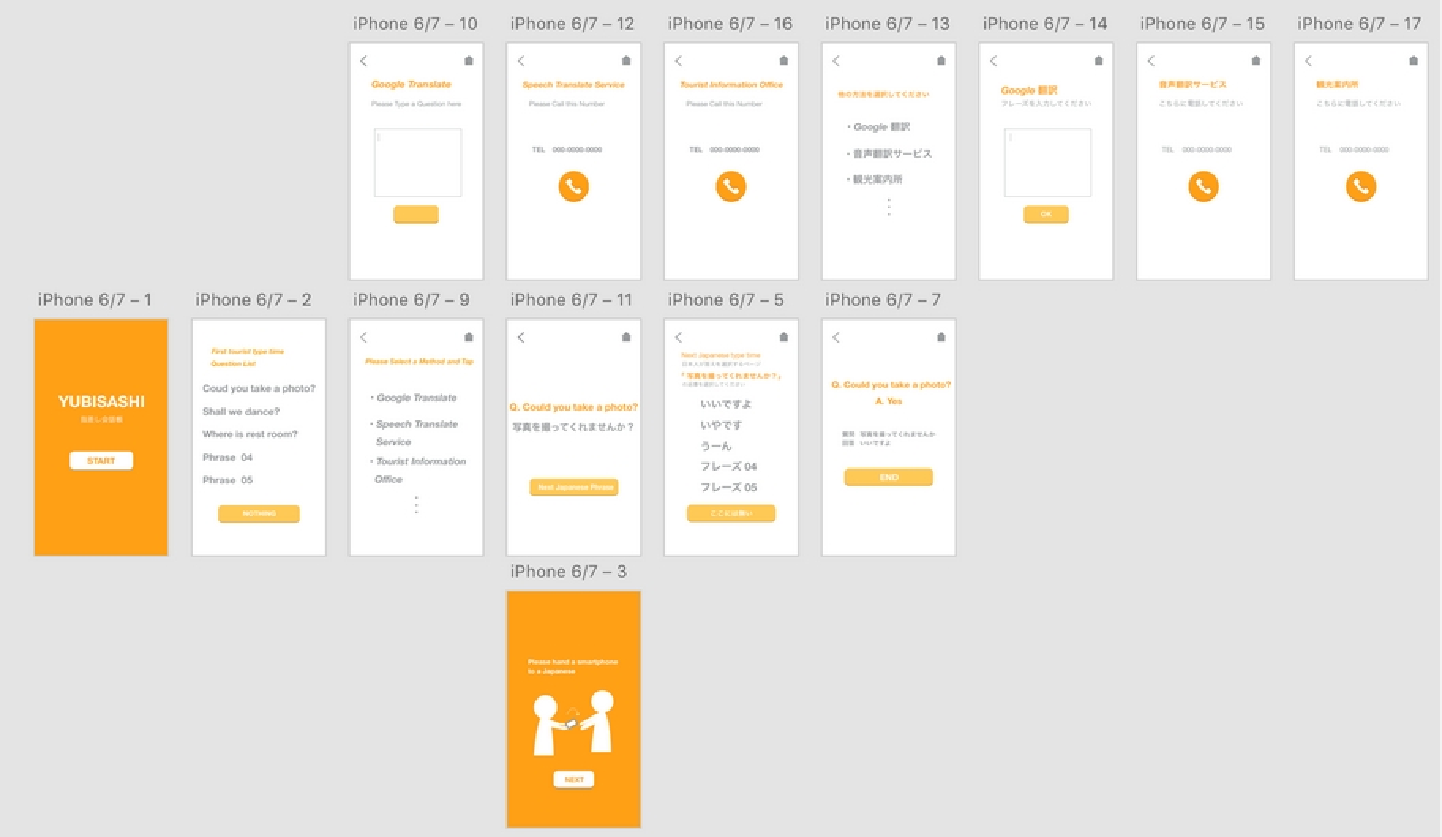
\includegraphics[width=10cm]{cde.pdf}\\
プロトタイプ
\end{center}
\bunseki{高橋大輔}


\chapter{中間報告会}

\section{発表形式}
 7月14日に行われた中間発表では、各グループの行ってきた活動を詳細に伝え、後期の活動に活かせるレビューを得ることを目的とした。発表としては, 全体のポスターを5分程度で発表し、その後に各グループごとに並列で7分程度の発表を行った。その後は時間の許す限り質疑応答の時間とした。私たちのグループでは、今回制作するアプリのモックアップをスマートフォン上に表示し、会話の流れをわかりやすくした。
\bunseki{荒田啓太郎}

\section{レビュー内容}

\subsection{発表方法についての評価と反省}
 中間発表会で行ったアンケートから非常に多かった意見が、言語対応が英語だけでは函館に来る外国人観光客でこのアプリを使えない人が出て来る為、多言語対応すべきというものだった。これは私たちの構想では多言語対応させるという案は上がっていたが、スクリプトやポスターには反映されていなかった為、このような意見が多数寄せられてしまった。よって、最終成果発表では多言語対応させたことについて明瞭に話し、誤解を招くような発表をしないように注意したい。
\bunseki{荒田啓太郎}

\subsection{発表内容についての評価と反省}
 中間発表会で行ったアンケートから最も多かったものが、本アプリをどうやって外国人観光客に認知してもらうのかというものであった。今回の発表をするにあたって本アプリは外国人観光客に入れておいてもらうのが前提としていた為、告知方法には力を注げていなかった。現状では、外国人観光客の多いであろう空港にビーコンでURLを送信するなどしか上がっておらず、後期では認知度をあげる手段についても深く検討していきたい。会話方法についても多くの意見をいただいた。このアプリは見知らぬ人に自身のスマホを渡す必要があり、そのことに対して不快感を覚えたり、手間だと考える人が非常に多いことがアンケートでわかった。他にも、外国人観光客に突然画面を見せられた時の日本人の反応や、回答を渋った場合の気持ちなど、本アプリでの会話方法には見直しが必要である。
そして、本アプリでは会話の成立のために事前にフレーズを用意して、外国人観光客が質問をする際、求めていたフレーズがなかった時に機械翻訳を用いるため、初めから機械翻訳を用いれば良いのではないかという意見をいただいた。また、指さし会話帳というものを参考にしているため、それらの手間を超えないようにする必要があるという意見もいただいた。これらについては私たちも考えていたことである。現状、機械翻訳との差別化として、機械翻訳の手間を省くためのフレーズを用意してあるので、もしも求めていたフレーズがあれば機械翻訳を通すまでもなく日本人と会話ができ、日本人用に用意された回答があるため会話がスムーズに進む点が挙げられる。しかしフレーズがない場合の対処方法が普通の翻訳と変わりないのでそこをどうするのか考えていく必要がある。指さし会話帳については、書籍の指さし会話帳に必要な調べるという手間を省くという目的があるので、フレーズの提案方法については吟味していきたい。
 これらの意見をまとめ、最終成果発表までに解決していくものを以下に記述した。
\begin{itemize}
 \item 本アプリをどのようにして外国人観光客に入れてもらうかの手法の考察
 \item 会話のきっかけを生むことはできるが会話を成立させるための工夫
 \item 機械翻訳や、指さし会話帳との差別化のためのUI設計やシステム構成
\end{itemize}
\bunseki{荒田啓太郎}


\chapter{グループBのプロセス}

\section{前期の活動}
  前期の活動では、はじめに函館市内で町に関するフィールド調査を行い、函館の問題点を見つけた。アイデア出しをする事前学習として、各自ビーコンについて調べ、他の人と内容を共有するプレゼン大会を行った。その後、今回ビーコンを提供していただくTangerine株式会社から、ビーコンのレクチャー会を開いてもらい、ビーコンの機能や過去に行ったビーコンを用いた事業例を学んだ。ビーコンの特徴を学んだ後、提案するサービスのアイデア出しを行い、そこで決まった3つのアイデアからそれぞれの班に分かれてサービスの詳細を決めていった。また、函館市のものづくり企業紹介の場に参加して、企業の方たちに私たちの活動を紹介したり、企業の活動を知るなどの交流会を行った。最後に、前期の活動の集大成として中間発表会でこれまでの活動内容を発表した。
\bunseki{河田歩美}

\section{今後の予定}
 ここでは後期の予定について紹介する。まず初めに制作の流れとしては、提案した案の見直しをして、簡単なプロトタイプを作り、そのあとにアプリケーション開発を進めていく。開発し終ったあとは、作ったアプリケーションを実際に使用してもらい、そのフィードバックから改善を行っていく予定である。
次にプロセスに沿って詳しい説明をしていく。後期の初めに、前期の中間発表で提案したアイデアに、発表を聞いていただいた方々のフィードバックを取り入れ、提案の改善を行っていく。次に、改善した内容を基にシステムを作っていく。制作については、スマートフォンアプリケーションを制作していく。私たちが提案するサービスは、~\ref{sec:sannosan}~にかかれてある通り、外国人を対象としたアプリケーションであるが、函館に観光しに来る外国人がどのスマートフォンを使っているかが想定できないため、AndroidとiOSの両方に対応したアプリケーションを作っていくことを予定している。アプリケーションの制作は、開発を行う前にメンバー同士の考えに相違点が生じないようプロトタイプを作って、内容を確認し合ってから開発を行おうと思っている。アプリケーションを制作した後、実際に函館市内にいる外国人観光客と市内に住む日本人に使用してもらい、使った感想や改善した方がいい点を聞き、再びアプリケーションの改善を行う。アプリケーションの改善と実際に使用してもらうことを何度か繰り返し行うことによって、私たちの提案するサービスの完成度を上げていきたいと思う。
\bunseki{河田歩美}


\chapter{前期の振り返りと学び}

\section{振り返り}

\subsection{スケジュール管理}
 スケジュール管理については、プロジェクト開始時に決定した年間スケジュールを元に管理を行った。
前期での活動では、年間スケジュールと概ね一致した活動や成果を出せた為、管理を行えていたといえる。
しかし、問題点としてスケジュール管理者が制作したスケジュールを早い段階から全体に公開していなかった事が挙げられる。
これによって、メンバーの多数が今自分が何をやっているのかについての理解に時間を要してしまった。
後期のプロジェクトでは、これを改善し、スケジュール管理者とメンバーとの意思疎通や、意見交換会を実施することで認識の齟齬を無くすことが重要であるといえる。
\bunseki{橋場保鷹}

\subsection{情報共有}
 私たちは、本プロジェクトが始まった当初、議題に対してプロジェクト全体で発表や共有、意見の交換を行っていた。
しかし、大人数で作業を行う際、アウトプットされる意見が少なかったり、情報伝達が行き届いていなかったりといった問題点があった。
そこで、私たちは3人から4人の小グループを作り、そこで討論を行なうといった手法を用いた。
人数を絞ることで個人が意見を出しやすい環境を作り、議論の効率化を図ったことにより、
より多くの意見をアウトプットさせることが出来た。
よって、私たちが後期のプロジェクト学習を行うに当たって、
小グループでのディスカッションを多く取り入れることが今後も重要になってくると考えられる。
\bunseki{橋場保鷹}

\section{学び}

\subsection{システム設計}
 私たちは、前期のプロジェクトを通してより実践的にどのようにしてシステムを設計するのかを学ぶことが出来た。
プロジェクト内でシステム設計についての考え方や、有用性のレクチャーを行ない、
本学の講義であるソフトウェア設計で学んだ技術を用いて実際に提案したサービスの設計を行った。
実際に自身で考えたサービスにシステムを肉付けしていくといった段階を踏んだ事により、
全体を通してより実践的なシステム開発技術を習得できたといえる。
\bunseki{橋場保鷹}

\subsection{情報をアウトプットする技術}
 私たちは、前期のプロジェクトを通して積極的に情報のアウトプットを行ってきた。
ブレーンストーミングやアイデアソンを通して、メンバー個人が保有している情報や発想を洗い出しを行った。
また、外部企業を招いてのアイデアコンテストや、函館市のものづくり企業紹介の場へ参加し、
自らの提案を積極的に外部へアウトプットした。
これらの経験により、プレゼンテーションを行うスキルや、内部情報を知らない外部の関係者がどのような情報を必要としているのかを知ることができ、
その情報をメンバー間で共有することで全体としてアウトプット技術の向上を図ることが出来た。
\bunseki{橋場保鷹}

% 以降、付録(付属資料)であることを示す
\begin{appendix}

\chapter{中間報告会で使用したグループBのポスター}
\begin{center}
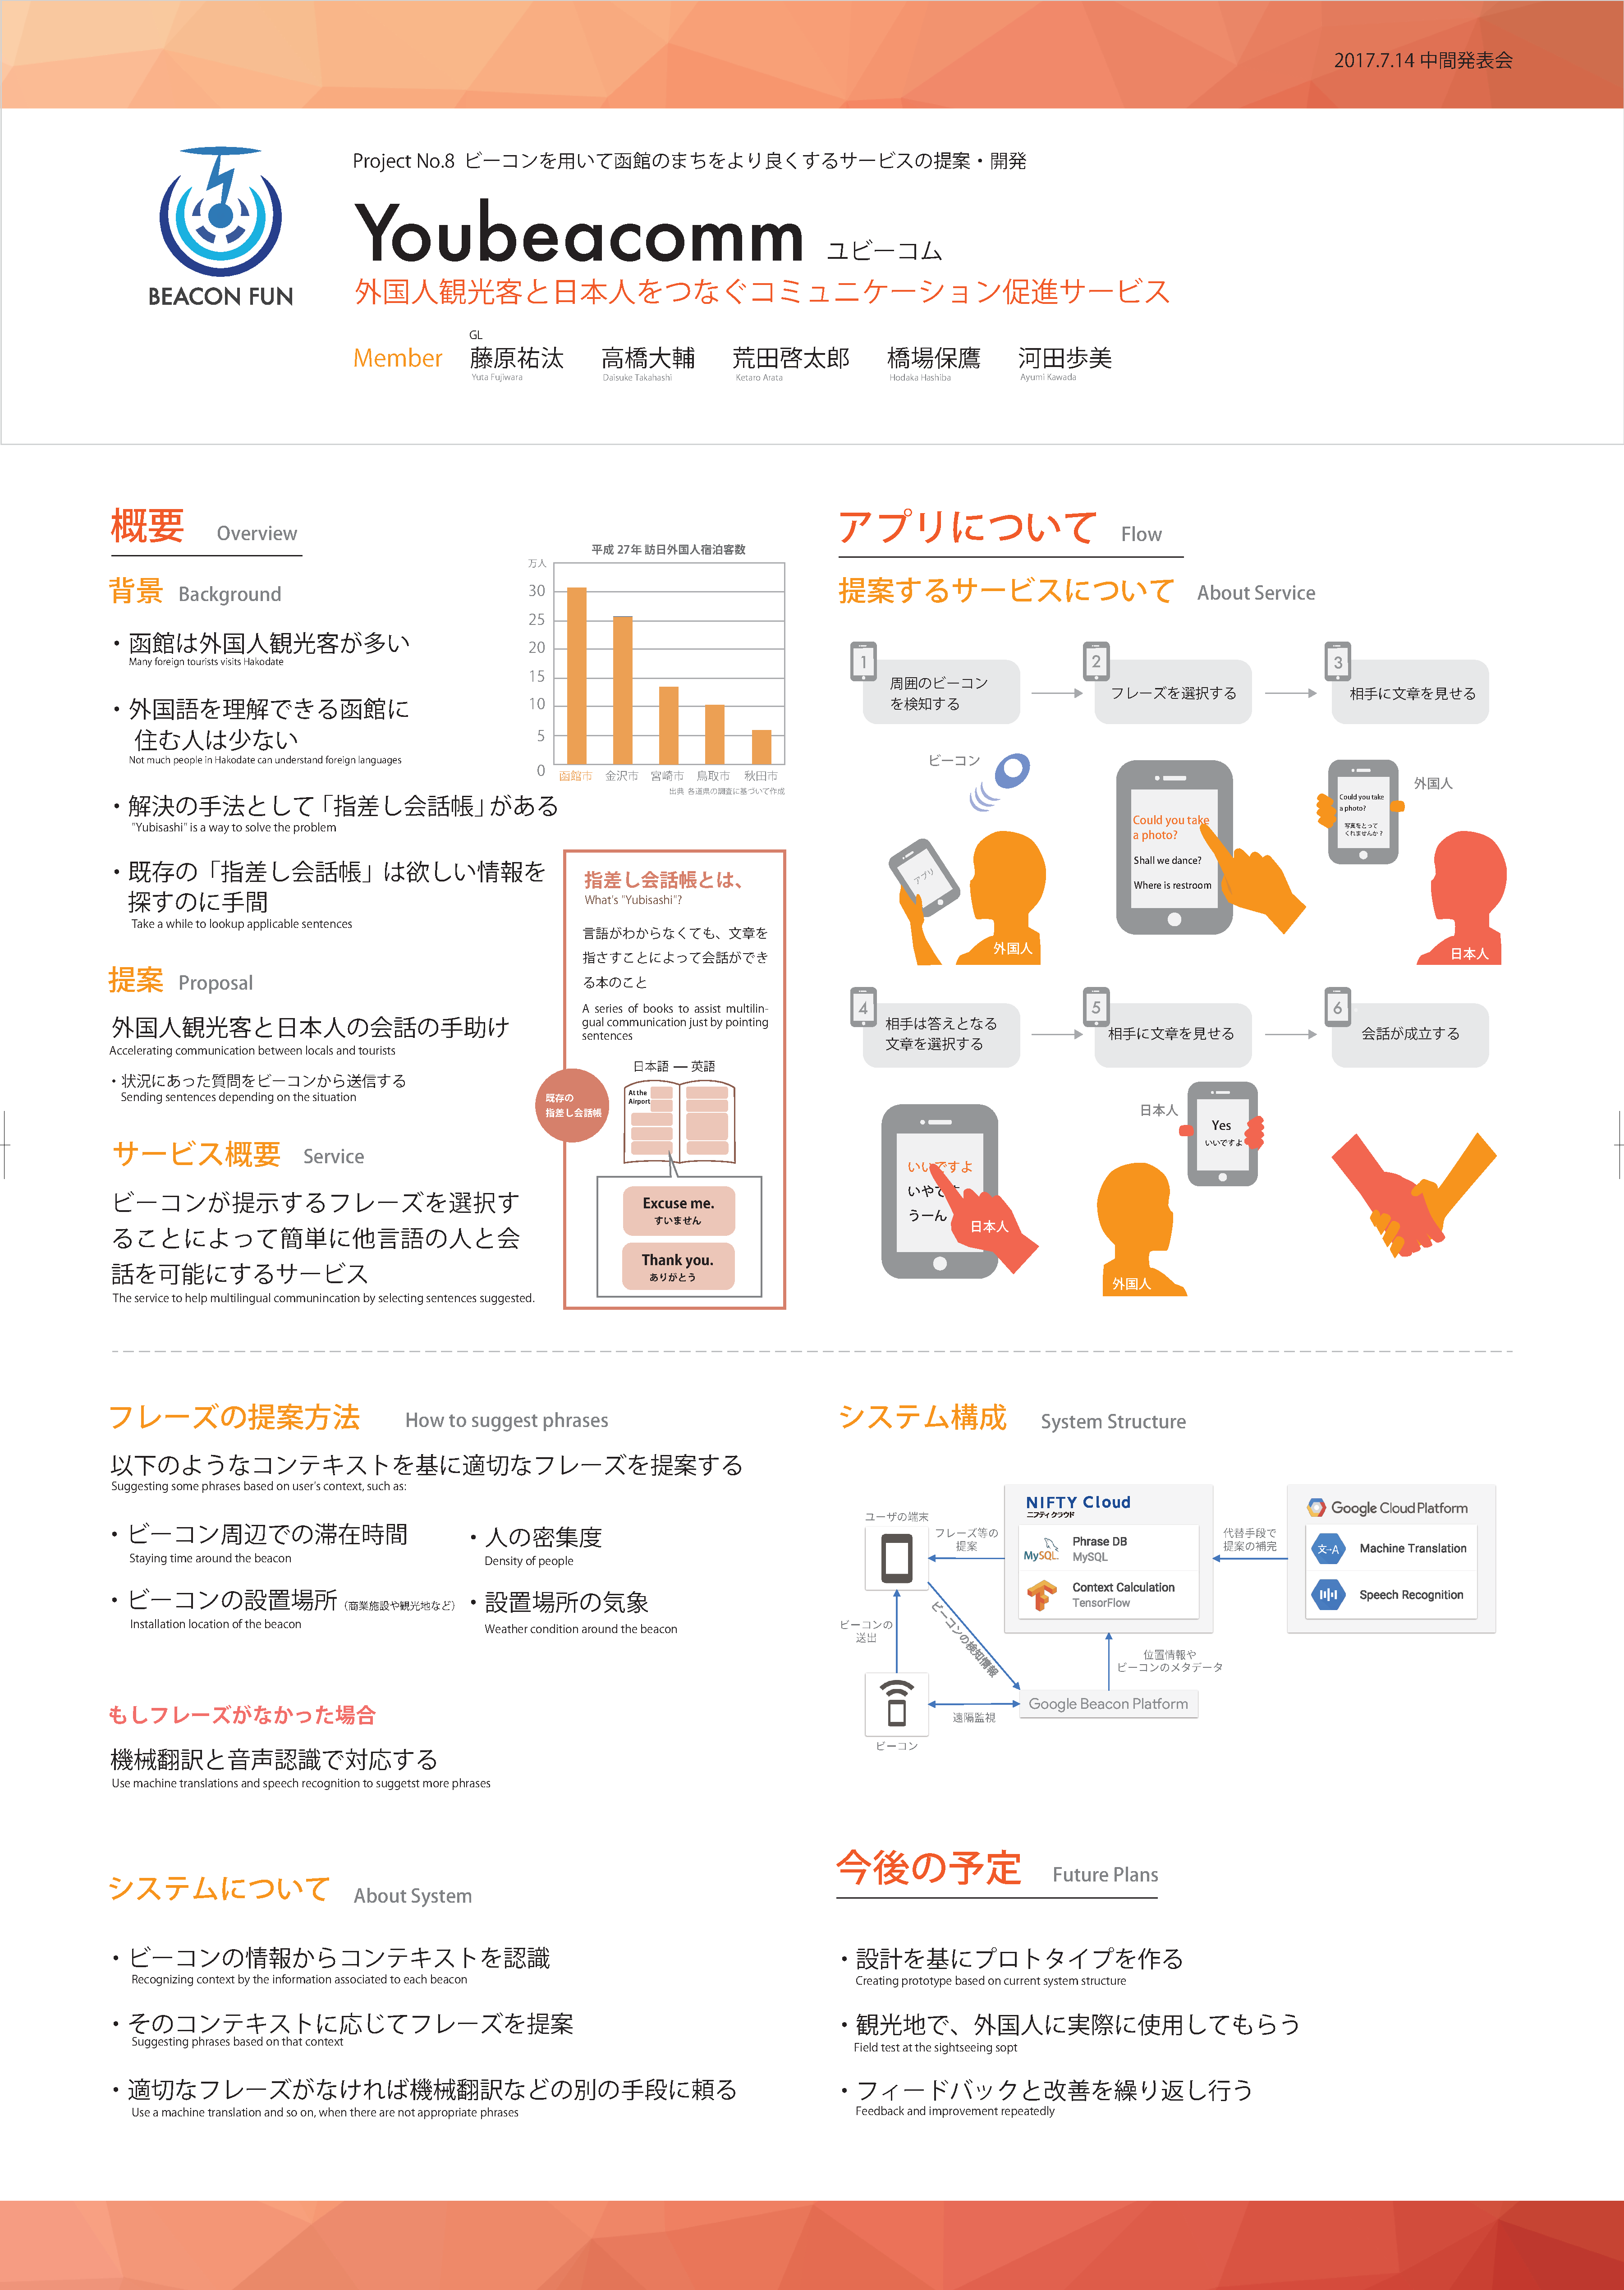
\includegraphics[width=13cm]{gbt.pdf}
\end{center}

%付録の終わり
\end{appendix}


%\backmatter

% 参考文献
\begin{thebibliography}{9}
\bibitem{a}総務省 平成28年版 情報通信白書 第1部 特集 IoT・ビッグデータ・AI~ネットワークとデータが創造する新たな価値~
 (http://www.soumu.go.jp/johotsusintokei/whitepaper/ja/h28/html/nc122530.html)

\bibitem{b}函館市観光部観光企画課 「来函観光入込客数推計」による。
(http://www.city.hakodate.hokkaido.jp/docs/2015062500021/files/H28irikomi.pdf)

\bibitem{c}米Net Applications社の調査による。
(https://www.netmarketshare.com/operating-system-market-share.aspx?qprid=8\&qpcustomd=1, 2017年7月20日閲覧)
 %\bibitem {ラベル} 著者名. 書籍名. 出版社,  年号.
 %\bibitem {A2} ほげほげお. うんたらかんたら,  2003.
\end{thebibliography}

\end{document}
